\section{Experiment 9M: unified confirmation-fleet ablation}
\label{sec:experiment9m}

\paragraph{Purpose and protocol.}
Experiment 9M reconstructs the principal baselines under one matched protocol
on the ten Experiment 9K fleets. It is a retrospective ablation of already
executed confirmation fleets, not a second blind confirmation. A freeze guard
requires the 9K clients, data volumes, identification settings, nonlinear
scenarios, mixture candidates, and federated settings. No model or controller
hyperparameter is retuned.

GlobalK1 shares one fleet-wide parameter vector and ignores heterogeneity.
LearnedCenter discovers an unknown number of groups but performs no continuous
personalization. CentralRank1/2 add one or two local coordinates to centralized
learned backbones. Fed20Rank1/2 learn the corresponding backbones from 20\%
random participation. OracleFamilyRank2 supplies the true generating family as
an unattainable diagnostic. Local fits all three parameters independently, and
ExactIndividual uses the true parameters.

Statistical comparisons first average all clients and scenarios within each
fleet. Ten independent fleet differences are then resampled 50000 times. This
fleet-level bootstrap avoids treating correlated trajectories or clients as
independent replicates. Reported intervals are percentile 95\% confidence
intervals for mean relative improvement.

\begin{table}[htbp]
\centering
\caption{Experiment 9M matched nonlinear tracking ablation.}
\label{tab:experiment9m-results}
\begin{tabular}{lrrrrr}
\toprule
Method & Local dim. & \multicolumn{2}{c}{0.75 s} & \multicolumn{2}{c}{1.25 s}\\
 & & Tracking & Param. err. & Tracking & Param. err.\\
\midrule
Local              & 3 & 0.012714 & 0.2063 & 0.007557 & 0.1197\\
GlobalK1           & 0 & 0.011544 & 0.1285 & 0.011544 & 0.1285\\
LearnedCenter      & 0 & 0.010826 & 0.0977 & 0.007798 & 0.0549\\
CentralRank1       & 1 & 0.010731 & 0.1007 & 0.007433 & 0.0499\\
CentralRank2       & 2 & 0.012709 & 0.1464 & 0.007530 & 0.0635\\
Fed20Rank1         & 1 & 0.010518 & 0.0976 & 0.007462 & 0.0520\\
Fed20Rank2         & 2 & 0.012774 & 0.1459 & 0.007562 & 0.0632\\
OracleFamilyRank2  & 2 & 0.012205 & 0.1322 & 0.007496 & 0.0533\\
ExactIndividual    & -- & 0.006664 & 0.0000 & 0.006664 & 0.0000\\
\bottomrule
\end{tabular}
\end{table}

\begin{figure}[htbp]
\centering
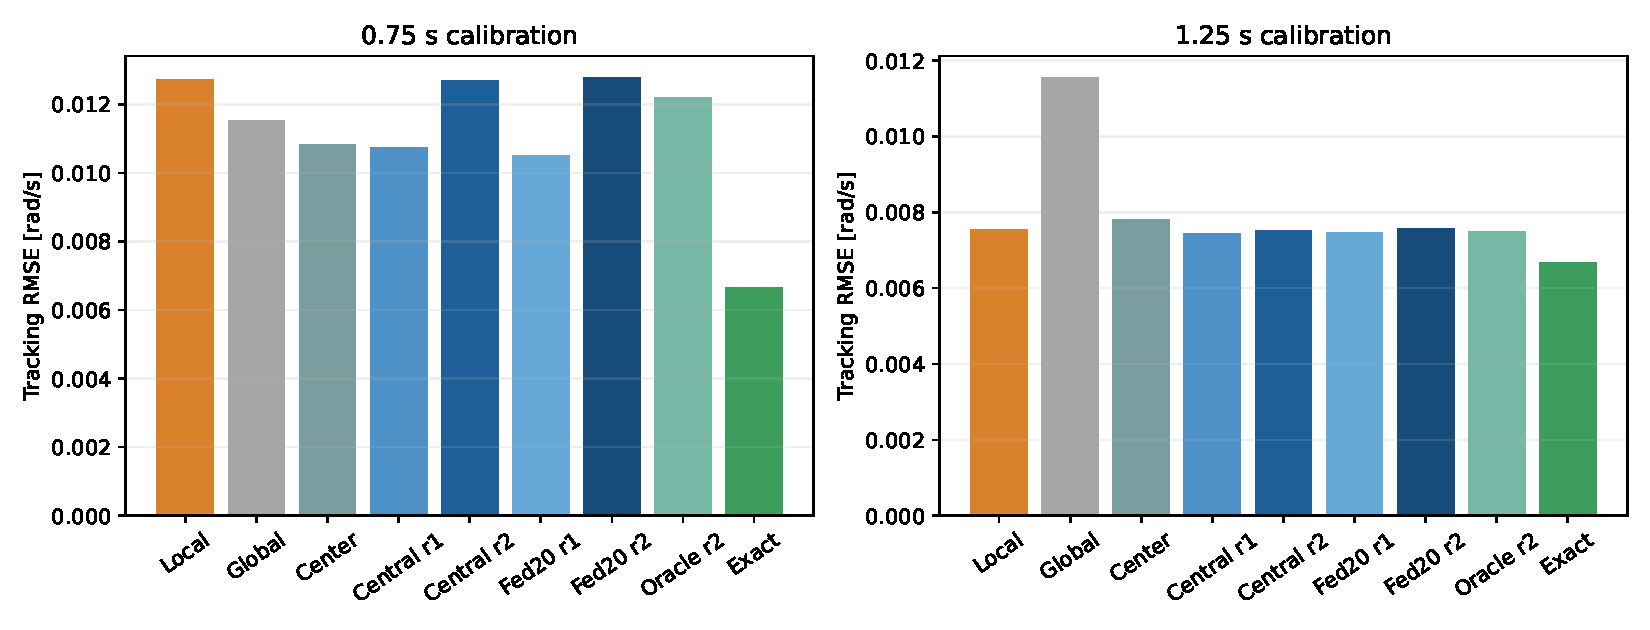
\includegraphics[width=0.95\linewidth]{../results/figures/experiment_9m_unified_ablation.pdf}
\caption{The matched ablation separates global sharing, discrete group
structure, continuous personalization, and distributed implementation.}
\label{fig:experiment9m}
\end{figure}

\begin{table}[htbp]
\centering
\caption{Fleet-level paired bootstrap analysis. Positive values favor the first
method.}
\label{tab:experiment9m-statistics}
\begin{tabular}{llrrr}
\toprule
Budget & Comparison & Mean & 95\% CI & Wins\\
\midrule
0.75 s & Fed20Rank1 vs. Local & 16.90\% & [11.79, 21.10]\% & 9/10\\
0.75 s & LearnedCenter vs. Local & 14.47\% & [9.73, 19.48]\% & 10/10\\
0.75 s & GlobalK1 vs. Local & 8.43\% & [2.50, 14.57]\% & 6/10\\
0.75 s & LearnedCenter vs. GlobalK1 & 5.95\% & [-0.44, 11.66]\% & 7/10\\
0.75 s & Fed20Rank1 vs. LearnedCenter & 2.20\% & [-4.56, 8.79]\% & 6/10\\
1.25 s & Fed20Rank1 vs. LearnedCenter & 4.21\% & [2.40, 6.36]\% & 10/10\\
1.25 s & Fed20Rank2 vs. Local & -0.06\% & [-0.71, 0.58]\% & 5/10\\
1.25 s & Fed20Rank1 vs. Fed20Rank2 & 1.17\% & [-1.27, 3.54]\% & 6/10\\
\bottomrule
\end{tabular}
\end{table}

\paragraph{Cold-start decomposition.}
At 0.75~s, even one global fleet model improves Local by 8.43\%, although it
wins only six fleets. Learned group centers improve Local by 14.47\%, win all
ten fleets, and have a confidence interval bounded away from zero. Thus the
dominant cold-start mechanism is a heterogeneous fleet prior, not estimation of
continuous client coordinates.

Fed20Rank1 improves Local by 16.90\%, confirming the 9K headline with a
fleet-bootstrap interval of 11.79--21.10\%. Its incremental 2.20\% improvement
over LearnedCenter is uncertain: the interval spans zero and it wins six
fleets. The paper must therefore not attribute the entire cold-start gain to the
personalized head. Federation itself incurs no observed penalty here:
Fed20Rank1 is 1.95\% better than CentralRank1, with a 0.70--3.18\% interval;
this favorable difference is treated as finite-sample cohort variation rather
than a general advantage of partial participation.

\paragraph{Personalization with increasing information.}
At 1.25~s, the group center alone is no longer competitive with Local, whereas
Fed20Rank1 improves the center by 4.21\%, wins all ten fleets, and has a
2.40--6.36\% interval. The role of the local head therefore emerges as the
client obtains enough information to move reliably within the fleet-supported
subspace. Fed20Rank1 is 1.12\% better than Local on average, but its interval
includes zero; this is parity rather than confirmed superiority.

Rank two is unnecessary in this matched analysis. At 0.75~s it overfits and is
approximately as poor as Local. At 1.25~s it is non-inferior to Local within the
chosen 1\% margin, but rank one has lower mean tracking and the rank-order
interval contains zero. Experiment 9H showed only a small development advantage
for rank two at 1.25~s; that ordering does not replicate. The robust conclusion
is that a very low-dimensional head suffices, not that rank two is required.

\paragraph{Scientific interpretation.}
The unified evidence supports a staged personalized-FL mechanism. Discrete
group structure supplies a useful prior immediately; one local coordinate then
adapts that prior when more client excitation becomes available. This is more
precise than claiming generic personalization superiority. Central learns
exactly three groups with ARI 1.000; Fed20 selects 3.1 groups on average with
ARI 0.917 and 99.94\% cumulative coverage, yet preserves the control result.

Both retrospective statistical gates pass: the Fed20Rank1 cold-start interval
excludes zero, and Fed20Rank2 at 1.25~s is non-inferior to Local under the 1\%
margin. Because the confirmation outcomes were already known before this
ablation was specified, these intervals quantify consistency and uncertainty;
they must not be presented as newly preregistered confirmatory tests. All 2400
fits converge and all 16200 nonlinear evaluations remain feasible.

\paragraph{Reproducibility.}
The matched configuration is in \path{code/config/experiment_9m.json}; the
driver and fleet-level bootstrap are in
\path{code/experiments/experiment_9m_unified_ablation.py}. Aggregate, seed-level,
cluster, statistical, and provenance records are stored under
\path{results/tables}.
